% REVISÃO DE LITERATURA--------------------------------------------------------

\chapter{Embasamento teórico }
\label{chap:embasamentoTeorico}

Este capítulo apresenta uma breve fundamentação dos assuntos e conceitos necessários para a melhor compreensão deste trabalho, dando ênfase aos pontos mais relevantes para a compreensão das atividades realizadas.

A SEDES é uma seção responsável por implementar e realizar manutenções em ativos de TI do TRE-PB. Dessa forma ela se comporta como uma fábrica de software, seguindo rigorosos critérios no desenvolvimento de seus produtos, todos documentados em um modelo de desenvolvimento, visando a qualidade e segurança de seus produtos. Técnicas e tecnologias reconhecidas do mercado são utilizadas, dentre elas o algumas metodologias ágeis como SCRUM e KAMBAM, JAVA, ORACLE SQL.

\section{SCRUM}
\label{sec:embasamentoTeoricoSCRUM}

SCRUM é uma metodologia (ou processo) de desenvolvimento iterativo e incremental, utilizada também no gerenciamento e desenvolvimento de software de forma ágil.

\begin{citacao}
    O SCRUM assume-se como uma metodologia extremamente ágil e flexível, que tem por objetivo definir um processo de desenvolvimento interativo e incremental podendo ser aplicado a qualquer produto ou no gerenciamento de qualquer atividade complexa. \cite{Bissi2007}.
\end{citacao}

No SCRUM, os projetos são divididos em Sprints, que são ciclos, geralmente mensais, que representam o tempo no qual um determinado conjunto de atividades deve ser executado. Cada atividade ou funcionalidade a ser implementada no projeto são mantidas em uma lista, chamada de Product Backlog. Ao iniciar cada sprint é realizada uma reunião de planejamento, conhecida como Sprint Planning Meeting. Nessa reunião, o Product Owner, que é a pessoa que define o que está no Product Backlog, irá determinar as prioridades e a equipe irá discutir quais atividades ela será capaz de executar naquela sprint. A partir daí, a cada dia dessa sprint é feita uma reunião diária, geralmente realizada no início do dia, denominada de Daily Scrum.  Nessa reunião, cada membro da equipe informa o que fez no dia anterior, e são identificados impedimentos e são estabelecidas novas prioridades para o dia atual.

Ao término de uma sprint, a equipe apresenta o que foi implementado, em uma pequena reunião, chamada Sprint Review Meeting. Logo após, é feito um novo planejamento para a próxima Sprint, reiniciando o ciclo, conforme é ilustrado na \autoref{fig:figura-cicloSCRUM}.

\begin{figure}[!htb]
    \centering
    \caption{Exemplo do cliclo SCRUM}
    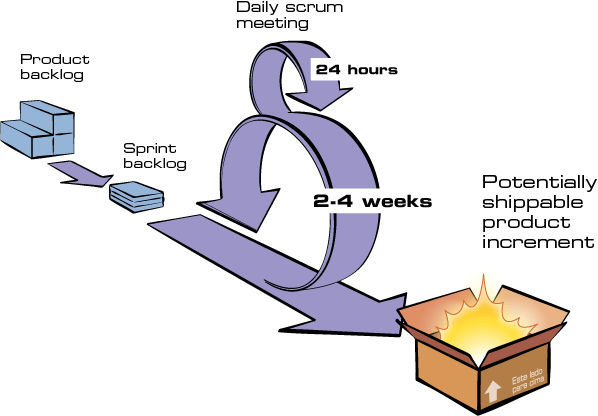
\includegraphics[width=0.5\textwidth]{./dados/figuras/cicloSCRUM}
    \fonte{teste..}
    \label{fig:figura-cicloSCRUM}
\end{figure}

Outro conceito do SCRUM é o Planning Poker, que é uma técnica utilizada para estimar o prazo de um projeto. Resumidamente, nessa técnica, é usado um conjunto de cartas. Cada carta contém um número que representa pontos. Os números vão de 1 a 100, seguindo a sequência 0, 1, 2, 3, 5, 8, 13, 20, 40, 100. Cada membro da equipe recebe o conjunto de cartas. Escolhido um ticket (tarefa), os usuários ao mesmo tempo lançam à mesa a carta com a quantidade de pontos que consideram que vale aquele ticket (geralmente, e esse foi o nosso caso, a quantidade de pontos remetia à quantidade de horas que levaríamos para executar aquela tarefa). O processo é repetido para todos os tickets. A ideia é instigar a discussão, pois, dificilmente, todos os membros da equipe irão jogar a mesma carta. Somente após um consenso é que o valor final é atribuído à tarefa \cite{Sabbagh2014}.

\section{Java}
\label{sec:embasamentoTeoricoJava}

Java\footnote{http://www.oracle.com/technetwork/pt/java/index.html} é uma linguagem de programação orientada a objetos, lançada em 1995, pela empresa Sun Microsystems, mas que, atualmente, pertence a Oracle \cite{Deitel2009}. A linguagem Java permite o desenvolvimento de software para as plataformas desktop (Standard Edition), mobile (Micro Edition) e web (Enterprise Edition). O código em Java não é compilado para código nativo, mas sim para um bytecode, que é executado por uma máquina virtual, a JVM (Java Virtual Machine). 
O Java é amplamente utilizado ao redor do mundo, principalmente em ambientes coorporativos. No Brasil, o Java é uma das principais linguagens de programação, sendo base para o ensino da Programação Orientada à Objeto na grande maioria dos cursos de programação. Além de ser bastante utilizada em organizações públicas. Isso se deve justamente pelo fato de que o foco do Java é em aplicações de médio a grande porte. Se forem bem usadas as recomendações e práticas do paradigma orientado à objeto, torna-se fácil a manutenção de uma aplicação Java, mesmo sendo de grande porte. Outra característica, que faz do Java uma ótima opção para esse escopo, é o suporte dela as diversas bibliotecas (ou APIs) para os mais diversos trabalhos como relatórios, persistência, gráficos, entre outras. 

\section{JSF}
\label{sec:embasamentoTeoricoJSF}

De acordo com \citeonline{Cordeiro2014}, JavaServer Faces\footnote{https://javaee.github.io/javaserverfaces-spec/}, ou, mais comumente, JSF, é um framework MVC para desenvolvimento web com Java, que veio para facilitar a construção de interfaces de usuário. A sua interface de usuário é baseada em componentes e orientada a eventos, sendo assim, os detalhes de manipulação dos eventos e a organização dos componentes são abstraídas. Com isso, o programador pode se concentrar bem mais na lógica do negócio. O JSF usa como sistema de template padrão o Facelets.

O JSF estabelece um conjunto de componentes pré-definidos para o desenvolvimento da interface de usuário. Para acessar esses componentes, ele fornece tags JSP. Outra característica interessante é que o JSF permite a reutilização dos componentes em uma página, aumentando a performance de carregamento da mesma. O JSF também faz uso do AJAX em alguns componentes, fazendo com que os processos sejam mais rápidos.

\section{PrimeFaces}
\label{sec:embasamentoTeoricoPrimeFaces}

PrimeFaces\footnote{https://primefaces.org/} é uma biblioteca Open Source de componentes para o JSF. Essa biblioteca contribui para que o software tenha, o que chamamos de interface rica, devido ao grande conjunto de componentes. O PrimeFaces utiliza o jQuery2 e jQuery UI. Assim como outros frameworks para a parte visual do sistema, ele também se preocupa com a responsividade do layout.
Os componentes do PrimeFaces foram construídos para usar AJAX por padrão, com isso o desenvolvedor não precisa ter a preocupação de realizar chamadas assíncronas para o servidor. O PrimeFaces também conta com um conjunto de temas (skins), que permite, de forma fácil mudar a aparência das aplicações.
A grande característica do PrimeFaces é a sua simplicidade. Não é necessário configurar nenhum XML. Para utilizá-lo, basta colocar a biblioteca no projeto. Tudo isso está muito bem documentado no site do PrimeFaces, que também possui vários exemplos de código \cite{Civici2015}.

\section{JPA}
\label{sec:embasamentoTeoricoJPA}

Java Persistense API\footnote{ http://www.oracle.com/technetwork/java/javaee/tech/persistence-jsp-140049.html} ou JPA é uma especificação criada em 2006 a partir do Hibernate\footnote{http://hibernate.org/}, que é um framework de mapeamento objeto-relacional (ORM), tendo em vista que outros frameworks estavam surgindo foi necessário criar um padrão com o intuito de resolver o famoso vendor lock-in, ou seja, uma vez usando determinada distribuição, ficava-se preso à mesma \cite[p.~12]{Cordeiro2014}.

A abstração do JPA é a sua maior característica, permitindo que o programador troque o banco de dados sem maiores dificuldades. No projeto \imprimirtitulo \space foi usado o Hibernate através da especificação JPA.O uso da JPA é feito através de anotações na classe que representa o objeto que será persistido. Esse processo de anotar/configurar classes chama-se mapeamento. As classes depois de mapeadas são reconhecidas pelo Hibernate, que faz o seu processo natural de converter esse objeto para uma tabela no banco de dados \cite{Cordeiro2014}.

\section{Hibernate}
\label{sec:embasamentoTeoricoHibernate}


\section{Spring Framework}
\label{sec:embasamentoTeoricoSpring}

O Spring surgiu em 2003 como uma resposta à complexidade das primeiras especificações do J2EE. Enquanto alguns consideram que Java EE e Spring estão competindo, o Spring é, de fato, complementar ao Java EE. O modelo de programação Spring não abrange a especificação da plataforma Java EE; em vez disso, integra-se com especificações individuais cuidadosamente selecionadas do JavaEE:

\begin{itemize}
    \item Servlet API (JSR 340)
    \item WebSocket API (JSR 356)
    \item Concurrency Utilities (JSR 236)
    \item JSON Binding API (JSR 367)
    \item Bean Validation (JSR 303)
    \item JPA (JSR 338)
    \item JMS (JSR 914)
\end{itemize}

O framework também suporta injeção de dependências (JSR 330)  e anotações comuns (JSR 250), que os desenvolvedores de aplicativos podem usar em vez dos mecanismos específicos do Spring.

\subsection{Anotações de Estereótipo}
São anotações usadas para declarar a função que o componente desempenha na aplicação. Por exemplo, a anotação @Repository no Spring Framework é uma marcação para qualquer classe que atenda a função de um repositório (também conhecido como Data Access Object ou DAO).

\section{JasperReports}
\label{sec:embasamentoTeoricoJasper}

O JasperReports é um framework open source inteiramente escrito em Java. Ele é um dos mecanismos mais populares para a geração de relatórios na plataforma Java.
O JasperReports nos fornece funcionalidades que permitem criar relatórios complexos de forma estruturada, a partir da elaboração de um template \cite{Devmedia2012}.

O template é um arquivo XML com a extensão .jrxml. É neste arquivo que é especificada a estrutura do relatório, ou seja, é nele onde informamos os dados que irão compor o relatório, em que posição e de que forma serão exibidos, formando assim um layout. Utiliza-se o IReports para diagramação dos elementos de maneira gráfica.

A partir da definição do template e com o auxílio do framework JasperReports é possível gerar relatórios e exportá-los para diversos formatos, como: HTML, PDF e DOC.

\section{Tomcat}
\label{sec:embasamentoTeoricoTomcat}

